\documentclass[12pt]{article}
\usepackage[english]{babel}
\usepackage[utf8x]{inputenc}
\usepackage{amsmath}
\usepackage{graphicx}
\usepackage{graphicx, lipsum,caption}
\usepackage[colorinlistoftodos]{todonotes}

\begin{document}
	
	\begin{titlepage}
		
		\newcommand{\HRule}{\rule{\linewidth}{0.5mm}} % Defines a new command for the horizontal lines, change thickness here
		
		\center % Center everything on the page
		
		%----------------------------------------------------------------------------------------
		%	HEADING SECTIONS
		%----------------------------------------------------------------------------------------
		
		\textsc{\LARGE Central Washington University}\\[1.5cm] % Name of your university/college
		\textsc{\Large Advanced Algorithms}\\[0.5cm] % Major heading such as course name
		\textsc{\large Winter 2019}\\[0.5cm] % Minor heading such as course title
		
		%----------------------------------------------------------------------------------------
		%	TITLE SECTION
		%----------------------------------------------------------------------------------------
		
		\HRule \\[0.4cm]
		{ \huge \bfseries Project 2 Report}\\[0.4cm] % Title of your document
		\HRule \\[1.5cm]
		
		%----------------------------------------------------------------------------------------
		%	AUTHOR SECTION
		%----------------------------------------------------------------------------------------
		
		\begin{minipage}{0.4\textwidth}
			\begin{flushleft} \large
				\emph{Author:}\\
				Hermann \textsc{Yepdjio} % Your name
			\end{flushleft}
		\end{minipage}
		~
		\begin{minipage}{0.4\textwidth}
			\begin{flushright} \large
				\emph{Professor:} \\
				Dr. Razvan \textsc{Andonie} % Supervisor's Name
			\end{flushright}
		\end{minipage}\\[1cm]
		
		% If you don't want a supervisor, uncomment the two lines below and remove the section above
		%\Large \emph{Author:}\\
		%John \textsc{Smith}\\[3cm] % Your name
		
		%----------------------------------------------------------------------------------------
		%	DATE SECTION
		%----------------------------------------------------------------------------------------
		
		{\large \today}\\ % Date, change the \today to a set date if you want to be precise
		
		%----------------------------------------------------------------------------------------
		%	LOGO SECTION
		%----------------------------------------------------------------------------------------
		
		
\includegraphics[width=12cm]{CWU-Logo.png}\\[.5cm] % Include a department/university logo - this will require the graphicx package
		
		%----------------------------------------------------------------------------------------
		
		\vfill % Fill the rest of the page with whitespace
		
	\end{titlepage}
	\newpage
	\tableofcontents
	\newpage
	
	
	
	\section{Introduction}
		The purpose of this project was to implement and compare different implementations of the merge sort algorithm from the book.
		
	\section {experimentation process}
		\begin{itemize}
			\item we implemented 4 different versions of the merge-sort algorithm
					\subitem -the multi-threaded MERGE\_SORT from  the textbook
					\subitem -the multi-threaded P\_MERGE\_SORT from the textbook
					\subitem -the sequential versions of both algorithms above
			\item C is the programming language we used along with the POSIX threads
			\item we generated 4 arrays of sizes 100, 1000, 10000 and 100000  and filled them up with random numbers, to test the implementations and we recorded the processing times for each implementation over each array.
		\end{itemize}
	\section{Results}
	{\centering
		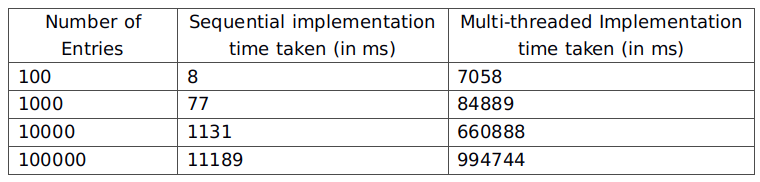
\includegraphics[width=\textwidth, height=10cm,keepaspectratio]{MERGE_SORT.png}
		\captionof{figure}{MERGE\_SORT(sequential(left) and multithreaded(right)\label{fig.1}}
	
		\par}
	\newpage
	{\centering
		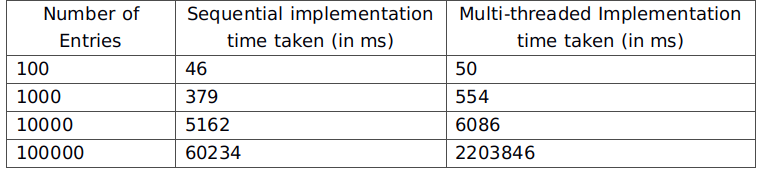
\includegraphics[width=\textwidth, height=10cm,keepaspectratio]{P_MERGE_SORT.png}
		\captionof{figure}{P\_MERGE\_SORT(sequential(left) and multithreaded(right)\label{fig.2}}
		
		\par}
	\section{Conclusion}
		From the tables above, we can see that
		\begin{itemize}
			\item the sequential version of MERGE\_SORT performs better than the sequential version of P\_MERGE\_SORT. This can be explained by the fact that the latter performs more computations than the first.
			\item the sequential version of MERGE\_SORT performs better than its multi-threaded version. This can be explained by the fact that it takes times to create the threads and also many of the threads will be created only to perform really simple operations such as sorting 1 or 2 numbers.
			\item the sequential version of P\_MERGE\_SORT performs better probably because of the same reasons described above.
			\item the multi-threaded version of P\_MERGE\_SORT is more efficient than the multi-threaded version of MERGE\_SORT probably because the merge operation is parallelized in the first. However, we also see that when the array gets bigger(array size = 100000), the multi-threaded MERGE\_SORT becomes faster. This is probably due to the fact that the number of threads created increases faster in the P\_MERGE\_SORT than in the MERGE\_SORT.
		\end{itemize}
			So  we can conclude that making a program multi-threaded does not necessary mean that the program will run faster especially if the threads will have to perform on a shared resource. In this case, a mechanism such as the use of mutex is needed to avoid the problem of race condition. Threads therefore have to wait for the resource to become available before they can do their job, which is time consuming and is not observed in the sequential implementation. 
	
\end{document}
